\documentclass[a4paper,10.5pt]{book}

\usepackage{babel}
\usepackage{lipsum}
\usepackage{hieroglf} % 添加古埃及象形文字
\usepackage{starfont} % 添加天文符号
\usepackage{pifont} % 添加 Dingbat
\usepackage{ccicons} % 添加 CC 协议
\usepackage{datetime}

\usepackage{chapterbib}

\usepackage[toc,page]{appendix}
\renewcommand{\appendixname}{附录}
\renewcommand{\appendixtocname}{附录}
\renewcommand{\appendixpagename}{附录}

\renewcommand\partname{}
\renewcommand\thepart{第 \arabic{part} 篇}
\renewcommand\bibname{参考文献}

\usepackage[top=1in,bottom=1in,left=1in,right=1in]{geometry} % 用于设置页面布局
\usepackage{xeCJK} % 用于使用本地字体
\usepackage[super, square, sort&compress]{natbib} % 处理参考文献
\usepackage{titlesec, titletoc} % 设置章节标题及页眉页脚
\usepackage{amssymb}
\usepackage{amsmath} % 在公式中用\text{文本}输入中文
\usepackage{diagbox}
\usepackage{multirow} % 表格中使用多行
\usepackage{booktabs} % 表格中使用\toprule等命令
\usepackage{rotating} % 使用sidewaystable环境旋转表格
\usepackage{tabularx}
\usepackage{graphicx} % 处理图片
\usepackage{footnote} % 增强的脚注功能,可添加表格脚注
\usepackage{threeparttable} % 添加真正的表格脚注,示例见README
\usepackage{hyperref} % 添加pdf书签

\usepackage{tikz}
\usetikzlibrary{shapes,arrows,shadows}


% 字体设置
\setmainfont{Times New Roman}
\setsansfont[Scale=MatchLowercase,Mapping=tex-text]{PT Sans}
\setmonofont[Scale=MatchLowercase]{PT Mono}
\setCJKmainfont[ItalicFont={STKaiti}, BoldFont={STHeiti}]{Songti SC}
\setCJKsansfont{Heiti SC}
\setCJKmonofont{Songti SC}

\newcommand{\song}{\CJKfamily{song}} % 宋体
\newcommand{\fs}{\CJKfamily{fs}} % 仿宋体
\newcommand{\kai}{\CJKfamily{kai}} % 楷体
\newcommand{\hei}{\CJKfamily{hei}} % 黑体
\newcommand{\li}{\CJKfamily{li}} % 隶书
\newcommand{\you}{\CJKfamily{you}} % 幼圆
\def\songti{\song}
\def\fangsong{\fs}
\def\kaishu{\kai}
\def\heiti{\hei}
\def\lishu{\li}
\def\youyuan{\you}

%%设置常用中文字号,方便调用
\newcommand{\chuhao}{\fontsize{42pt}{\baselineskip}\selectfont}
\newcommand{\xiaochu}{\fontsize{36pt}{\baselineskip}\selectfont}
\newcommand{\yihao}{\fontsize{26pt}{\baselineskip}\selectfont}
\newcommand{\xiaoyi}{\fontsize{24pt}{\baselineskip}\selectfont}
\newcommand{\erhao}{\fontsize{22pt}{\baselineskip}\selectfont}
\newcommand{\xiaoer}{\fontsize{18pt}{\baselineskip}\selectfont}
\newcommand{\sanhao}{\fontsize{16pt}{\baselineskip}\selectfont}
\newcommand{\xiaosan}{\fontsize{15pt}{\baselineskip}\selectfont}
\newcommand{\sihao}{\fontsize{14pt}{\baselineskip}\selectfont}
\newcommand{\xiaosi}{\fontsize{12pt}{\baselineskip}\selectfont}
\newcommand{\wuhao}{\fontsize{10.5pt}{\baselineskip}\selectfont}
\newcommand{\xiaowu}{\fontsize{9pt}{\baselineskip}\selectfont}
\newcommand{\liuhao}{\fontsize{7.5pt}{\baselineskip}\selectfont}
\newcommand{\xiaoliu}{\fontsize{6.5pt}{\baselineskip}\selectfont}
\newcommand{\qihao}{\fontsize{5.5pt}{\baselineskip}\selectfont}
\newcommand{\bahao}{\fontsize{5pt}{\baselineskip}\selectfont}

% 章节标题显示方式及页眉页脚设置
% \item xCJKnumb是自己额外安装的包
% \item titleformat命令定义标题的形式
% \item titlespacing定义标题距左、上、下的距离
\titleformat{\section}{\raggedright\large\bfseries}{\thesection}{1em}{}
\titleformat{\subsection}{\raggedright\normalsize\bfseries}{\thesubsection}{1em}{}
\titlespacing{\section}{0pt}{*2}{*0}
\titlespacing{\subsection}{0pt}{*1}{*0}

% 由于默认的2em缩进不够,所以我手动调整了,但是在windows下似乎2.2就差不多了,或者是article中没有这个问题
\setlength{\parindent}{2em}
\setlength{\parskip}{0.25em}

% 设置表格标题前后间距
\setlength{\abovecaptionskip}{0pt}
\setlength{\belowcaptionskip}{0pt}

% 设置列表项目前后间距
\setlength\itemsep{0em}

\renewcommand{\refname}{\bfseries{参~考~文~献}} %将Reference改为参考文献(用于 article)
% \renewcommand{\bibname}{参~考~文~献} %将bibiography改为参考文献(用于 book)

\renewcommand{\baselinestretch}{1.4} %设置行间距
\renewcommand{\figurename}{\small\ttfamily 图}
\renewcommand{\tablename}{\small\ttfamily 表}


\usetikzlibrary{shapes,arrows,positioning,decorations.pathreplacing,calc}

\newdateformat{monthyeardate}{\THEYEAR 年 \THEMONTH 月}

\makeatletter
    \def\subtitle#1{\gdef\@subtitle{#1}}
    \def\maketitle{
    \begin{titlepage}
        \begin{center}
            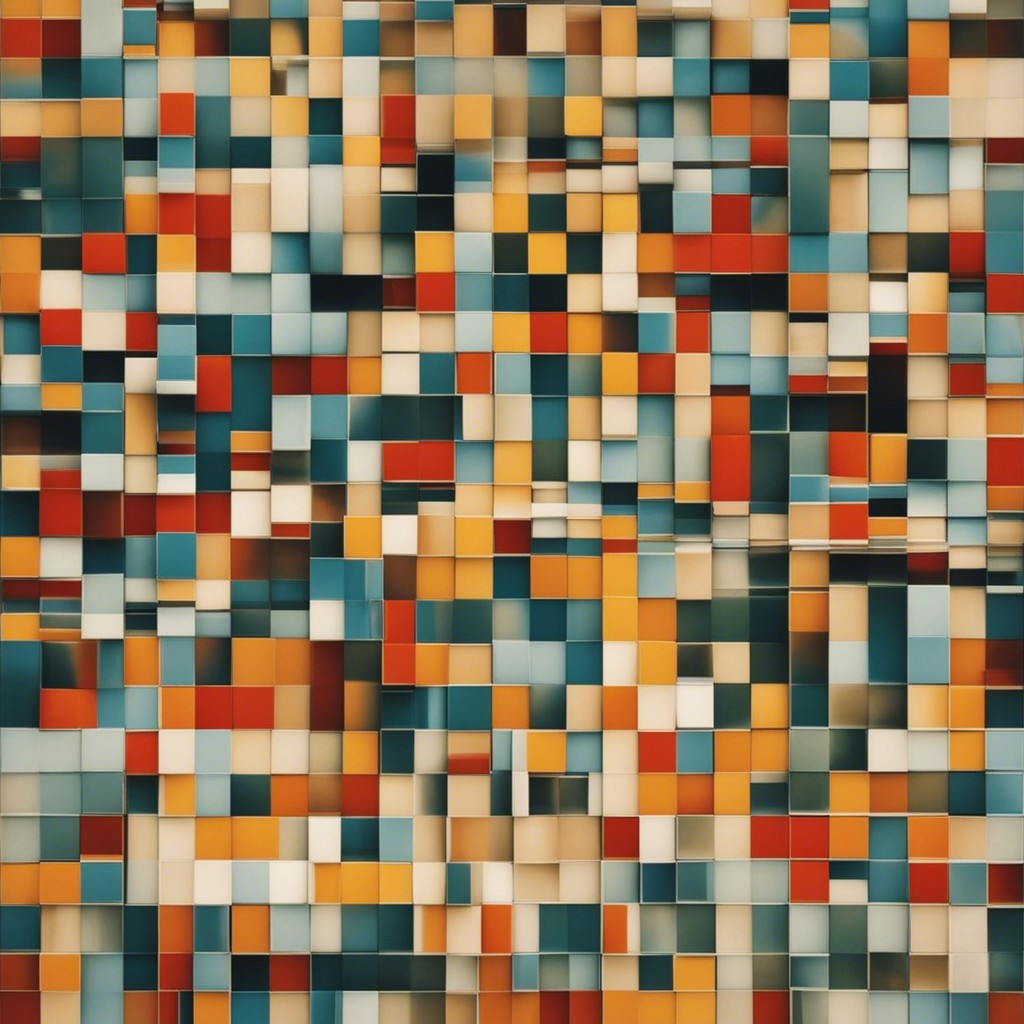
\includegraphics[width=6.5in]{images/00_00-Cover.jpeg}\\[5ex]
            {\yihao \bfseries  \@title }\\[10ex]
            {\erhao \bfseries  \@subtitle }\\[10ex]
            {\sanhao  \@author}\\[5ex]
            {\sihao \monthyeardate\today}\\[1ex]
        \end{center}
    \end{titlepage}
    }

\makeatother

\newcommand{\specialcell}[2][c]{%
  \begin{tabular}[#1]{@{}c@{}}#2\end{tabular}}

\titleformat{\chapter}[display]
  {\bfseries \sanhao}
  {第 \thechapter 章}
  {1ex}
  {\titlerule\vspace{1ex}\filleft}
  [\vspace{1ex}\titlerule]

\titlespacing{\chapter}{0pt}{*1}{*1.5}

\xeCJKsetwidth{‘’“”}{1em}

\usepackage[acronym,xindy]{glossaries}
\renewcommand*{\glossaryname}{索~引}
\makeglossaries

\usepackage[xindy]{imakeidx}
\makeindex

\loadglsentries[main]{glossary/glossary}

\setcounter{tocdepth}{1}

\pmhgfamily

\title{数学历史资料}
\subtitle{资料片段的整理}
\author{苑明理}
\date{}

\begin{document}
\thispagestyle{empty}
\newpage
%Add content for page two here (useful for two-sided printing)

\newpage
\thispagestyle{empty}
\maketitle
\begin{center}
    \copyright
\end{center}
\thispagestyle{empty}

\newpage

\setlength{\parindent}{0em}
\setlength{\parskip}{1.2em}

\chapter*{序言}

在波涛汹涌的洋面上,发光的浮游生物在黑暗的水域里飘动。它们的体内有发光物质,一旦感知到周围环境的变化时,这些发光物质就会被触发、闪烁,
仿佛黑暗中摇曳的点点星辰;它们相互呼应,把孤立的星辰连成一片星海。数学最为遥远的源头,可能就像这些浮游生物一样,
源自于生命对于自然界律动和模式的感知、反映与应答。

伴随着脑容量不断扩大,这种生命和环境的互动模式随着时间的推移和生物演化逐渐复杂化。从几亿年前的昆虫开始,动物已经开始展示出令人惊讶的数学能力。
此时承载数学能力的媒介是生物个体本身。数学的演化要通过生物的演化来实现,这种演化的速度是极其缓慢的。

更新世后期,伴随着智人语言能力的发展,这种原始的感知与能力借助符号的力量,终于脱离了身体的限制,开始不断加速迭代。
在这一阶段,承载数学能力的媒介是符号,数学开始成为一种跨越代际的文化现象。在几十万年的时间尺度内,数学的文化层层累进,发展成一棵参天大树。
它深刻地影响着人类的行为,塑造着人类的精神生活、制度规范和物质世界。


\newpage

\setlength{\parindent}{0em}
\setlength{\parskip}{0em}

\renewcommand\contentsname{目录}
\tableofcontents
\thispagestyle{empty}

\newpage

\setcounter{page}{1} %Start the actually document on page 1

\setlength{\parindent}{0em}
\setlength{\parskip}{1.2em}

\part{生物的数学能力}

\chapter{蚂蚁的数学}

作为当今世界上最为成功的物种之一,蚂蚁虽然只有大约 25 万个神经元细胞,但其复杂的生物学行为却令人瞩目。
特别是其归巢行为,已经成为了数学和生物学研究的重要课题。\cite{Wehner2003DesertAN}
这不仅证明了即使是“简单”的生物也具有出奇不意的数学能力,而且还为我们理解数学如何根植于自然界提供了宝贵的线索。

\begin{figure}[ht]\centering
\resizebox{0.5\textwidth}{!}{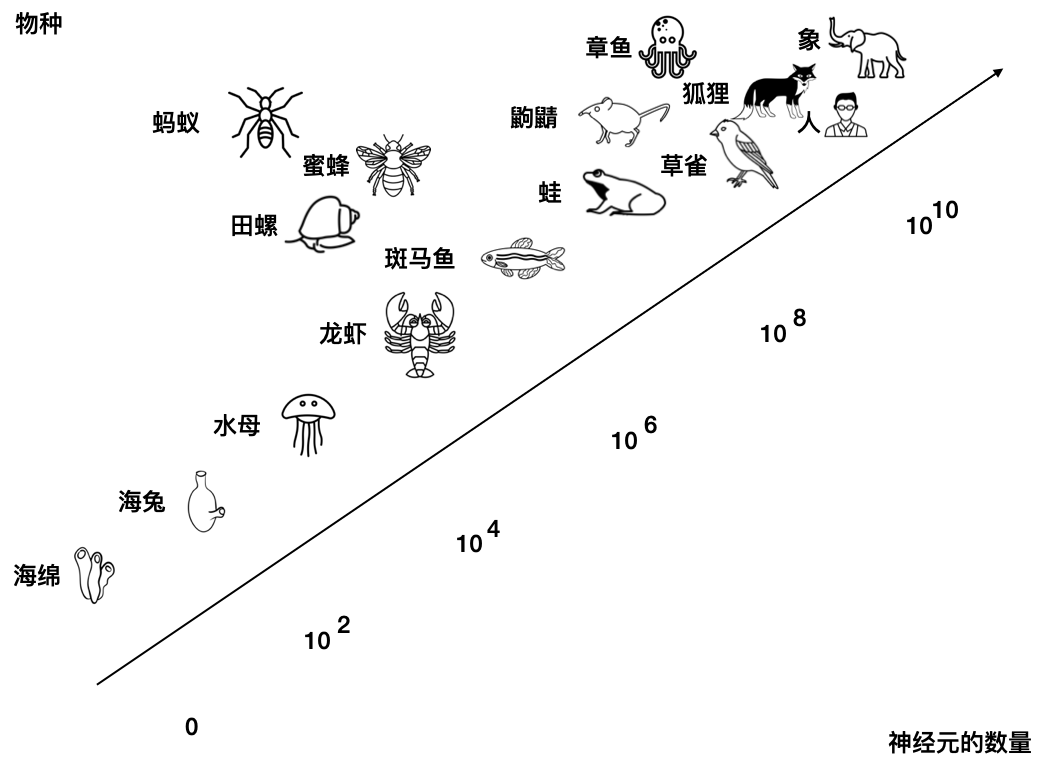
\includegraphics{images/01_01-species-neuron}}
\caption{物种与神经元数量}
\end{figure}

Wehner 等人在 2003 年的一项引人注目的实验中发现了令人惊讶的事实。沙漠蚁在归巢时,并不依赖于地理空间的绝对位置,
而是采用了一种被称为“路径积分”的策略。\cite{Wehner2003DesertAN}简而言之,这些蚂蚁会在移动过程中不断记录自己的方向和距离,
然后利用这些信息来确定回到巢穴的最直接路径。这一发现不仅展示了蚂蚁在数学方面的先天能力,也进一步证实了数学能力是生物界中普遍存在的现象。

在 Wehner 的实验 A 中,沙漠蚁在自由行走中会径直返巢。对照实验 B 则设置了挡板(图 \ref{fig:ant-navi} 中灰色线),沙漠蚁被挡板阻挡不得不绕行;但是一旦挡板消失,它们就会径直返巢。
我们能从实验 B 结果的图示上,清晰而直接地看到沙漠蚁有三角学角度的解算能力。
Wittlinger 在 2006 年的实验,也进一步说明沙漠蚁有计步能力。\cite{Wittlinger2006TheAO}
这些数学能力蕴含在生物的本能中,不是以符号的形式存在的。

\begin{figure}[ht]\centering
\resizebox{0.5\textwidth}{!}{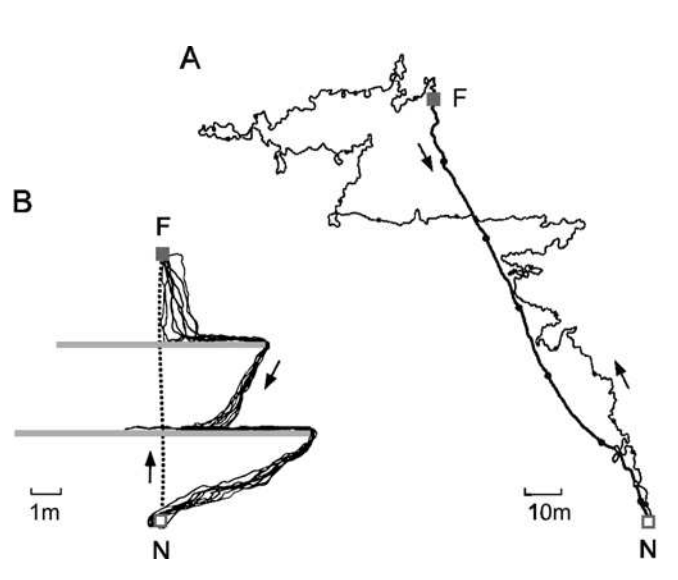
\includegraphics{images/01_02-ant-navi}}
\caption{关于蚂蚁归巢行为的实验}\label{fig:ant-navi}
\end{figure}

在导航能力的研究中,动物大脑的神经科学机制也是一个热门话题。科学家们已经区分了两种主要的动物导航原理:
一种是以自我为中心的导航(也就是“自我中心式的”或egocentric),另一种是依赖于外部地标的导航(也就是“地标式的”或geocentric)。
这两种导航方式背后都有复杂的神经科学机制。对于高等的动物,位置细胞和网格细胞在动物大脑中起到了关键作用,它们为动物提供了空间定位的神经科学基础
\cite{Moser2008PlaceCG}。这一发现不仅增加了我们对动物数学能力的理解,也为探究人类数学思维提供了新的视角。

从这些研究中,我们可以推测,人类数学的根源很可能是生物在数亿年的演化过程中逐渐形成的数学能力。
这种能力不仅仅是生物为了适应环境而演化出来的,它背后的神经机制还是我们数学直觉的基础。但这引出了一些更为引人入胜的问题:
人类的数学思维能否,以及如何,超越这种深植于我们基因的原始数学能力?人类原始的数学直觉是如何转化为更高级的数学概念,例如无穷、概率或者高维几何?
再如,我们是否可以,设计一个实验观察动物大脑在高维数字虚拟空间中的活动过程?这一类的探索不仅可以成为一个严肃的科学问题,
也触及了哲学和文化的多个层面,会帮助我们进一步理解人类数学思维和数学实在的本质。

\bibliographystyle{apalike2}
\bibliography{biblio/chp01}

\chapter{章鱼的数学}

\chapter{鸟类的数学}

\chapter{哺乳类的数学}

\chapter{认知心理学的进展}


\part{符号数学的开端}

\chapter{一进数制的建立}

\section{最早的符号}

如果人类演化是一幅巨大的动画作品,时间是流动的轴,而空间则是由各种文化、科技和社会因素组成的多彩色块。
在这幅动画中,每一个时间点都像是一个静止的剖面,其中的色块—比如散落的族群、火的采用、工具的制作、葬仪的方式、语言、音乐和艺术……—相互交织,
构成了一幅瑰丽的“镶嵌画”。

在 30 多万年前,智人出现在非洲,解剖学意义上他们已经具备现代性,甚至他们的大脑容量比我们还要大。大约在 5 万年前,人类开始进入一个新的阶段,
人类的文化开始爆炸性发展。这段历史被称为行为的现代性(Behavioral modernity)。

刻痕记事是最早的符号使用形式之一,它在数学发展中起到了催化作用。出土在刚果的、2 万年前的 Isango 骨刻是这一形式的现存最早证据,
它已经呈现出一种非常娴熟的运用(图 \ref{fig:isango})。符号使用可能比我们想象的还要早,甚至可能早于智人的出现,
这为数学的起源提供了更为久远的时间线。

虽然刻痕在早期人类生活中可能只是一个细小的部分,但它在数学的起源中占有不可或缺的地位。刻痕的抽象性和指代能力不仅是数学符号的基础,
也是数学思维从生物个体外化转变到符号的关键一步。从这个角度看,刻痕可以被视为一种原始的“1-进数”,它是数学从生物学现象演化到文化现象的一个重要里程碑。

\begin{figure}[ht]\centering
\resizebox{0.5\textwidth}{!}{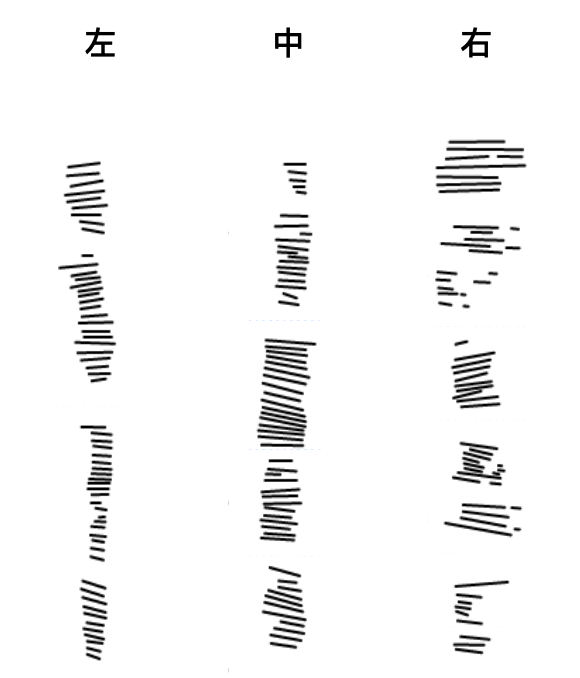
\includegraphics{images/01_03-isango-carved-bone}}
\caption{出土在刚果的 Isango 骨上的刻痕}\label{fig:isango}
\end{figure}

\section{有限性}

几乎可以肯定,当刻痕开始被人类熟练运用,其后不久的某一个时刻,一定有某个人会突然意识到:理论上,刻痕可以无穷无尽的排列下去。
如果历史真的这么展开,这会是人类第一次开始思考无穷的概念。这假想的时刻也将非常可能是“数”作为一个系统第一次登上历史舞台。

\section{一进数制的建立}

\chapter{多进数制}

\chapter{乘法的探讨}


\begin{appendices}
\chapter{附录一}

\lipsum[1-4]

\chapter{附录二}

\lipsum[1-4]

\end{appendices}

\chapter*{术语索引}

\phantomsection
\addcontentsline{toc}{chapter}{术语索引}

\printindex
\printglossaries
\newpage


\chapter*{参考文献}

\phantomsection
\addcontentsline{toc}{chapter}{参考文献}

\bibliography{biblio/book}

\newpage



\end{document}
